\documentclass[tikz,border=8pt,multi=tikzpicture]{standalone}
\usepackage{fontspec}
\setsansfont{TeX Gyre Heros}
\renewcommand{\familydefault}{\sfdefault}
\usepackage{tikz}
\usetikzlibrary{arrows.meta,positioning,calc}
\definecolor{ink}{HTML}{172B45}
\definecolor{muted}{HTML}{52647A}
\definecolor{line}{HTML}{CBD5E1}
\definecolor{paper}{HTML}{F3F6FA}
\definecolor{indigo}{HTML}{4338A0}
\definecolor{indigopale}{HTML}{EFEDFA}
\definecolor{teal}{HTML}{076C68}
\definecolor{tealpale}{HTML}{EAF6F3}
\tikzset{
  every node/.style={font=\sffamily\fontsize{12}{16}\selectfont,text=ink},
  box/.style={draw=line,fill=white,rounded corners=5pt,line width=.7pt,
    text width=4.8cm,minimum height=1.9cm,align=center,inner sep=10pt},
  coordinator/.style={box,draw=indigo,fill=indigopale,line width=1.2pt},
  tool/.style={box,draw=teal,fill=tealpale},
  link/.style={{Latex[length=2.5mm]}-{Latex[length=2.5mm]},draw=muted,line width=.9pt},
  label/.style={font=\sffamily\fontsize{10}{13}\selectfont,text=muted,align=center},
  heading/.style={anchor=west,font=\sffamily\bfseries\fontsize{10}{12}\selectfont,text=muted},
}
\newcommand{\framebase}[3]{%
  \path[use as bounding box] (0,0) rectangle (25,15.3);
  \fill[white] (0,0) rectangle (25,15.3);
  \node[heading,text=indigo] at (.3,14.9) {CODEX / DOS FORMAS DE ORGANIZAR EL TRABAJO};
  \node[anchor=west,font=\sffamily\bfseries\fontsize{25}{29}\selectfont] at (.3,13.95) {#1};
  \node[anchor=west,text=muted] at (.3,13.15) {#2};
  \fill[paper,rounded corners=5pt] (.3,11.8) rectangle (24.7,12.6);
  \node[anchor=west,font=\sffamily\fontsize{11}{14}\selectfont] at (.6,12.2)
    {MISMA TAREA\quad Leer \texttt{ventas.csv} y generar \texttt{grafico.png} en OCI.};
  \fill[paper,rounded corners=7pt] (.3,3.25) rectangle (5.2,11.35);
  \fill[paper,rounded corners=7pt] (5.5,3.25) rectangle (14.8,11.35);
  \fill[paper,rounded corners=7pt] (15.1,3.25) rectangle (24.7,11.35);
  \node[heading] at (.65,10.9) {PUNTO DE ENTRADA};
  \node[heading] at (5.85,10.9) {TU MÁQUINA EN OCI};
  \node[heading] at (15.45,10.9) {OPENAI};
  \node[anchor=west,text width=23.5cm,font=\sffamily\fontsize{10}{13}\selectfont,text=muted]
    at (.3,.65) {Esquema conceptual, no prueba ejecutada. Flechas dobles: intercambio de mensajes.\quad #3\enspace / 02};
}
\newcommand{\takeaway}[2]{%
  \fill[indigopale,rounded corners=5pt] (.3,1.4) rectangle (24.7,2.8);
  \node[anchor=west,text=indigo,font=\sffamily\bfseries\fontsize{12}{15}\selectfont] at (.65,2.35) {#1};
  \node[anchor=west,font=\sffamily\fontsize{11}{14}\selectfont] at (.65,1.82) {#2};
}
\begin{document}
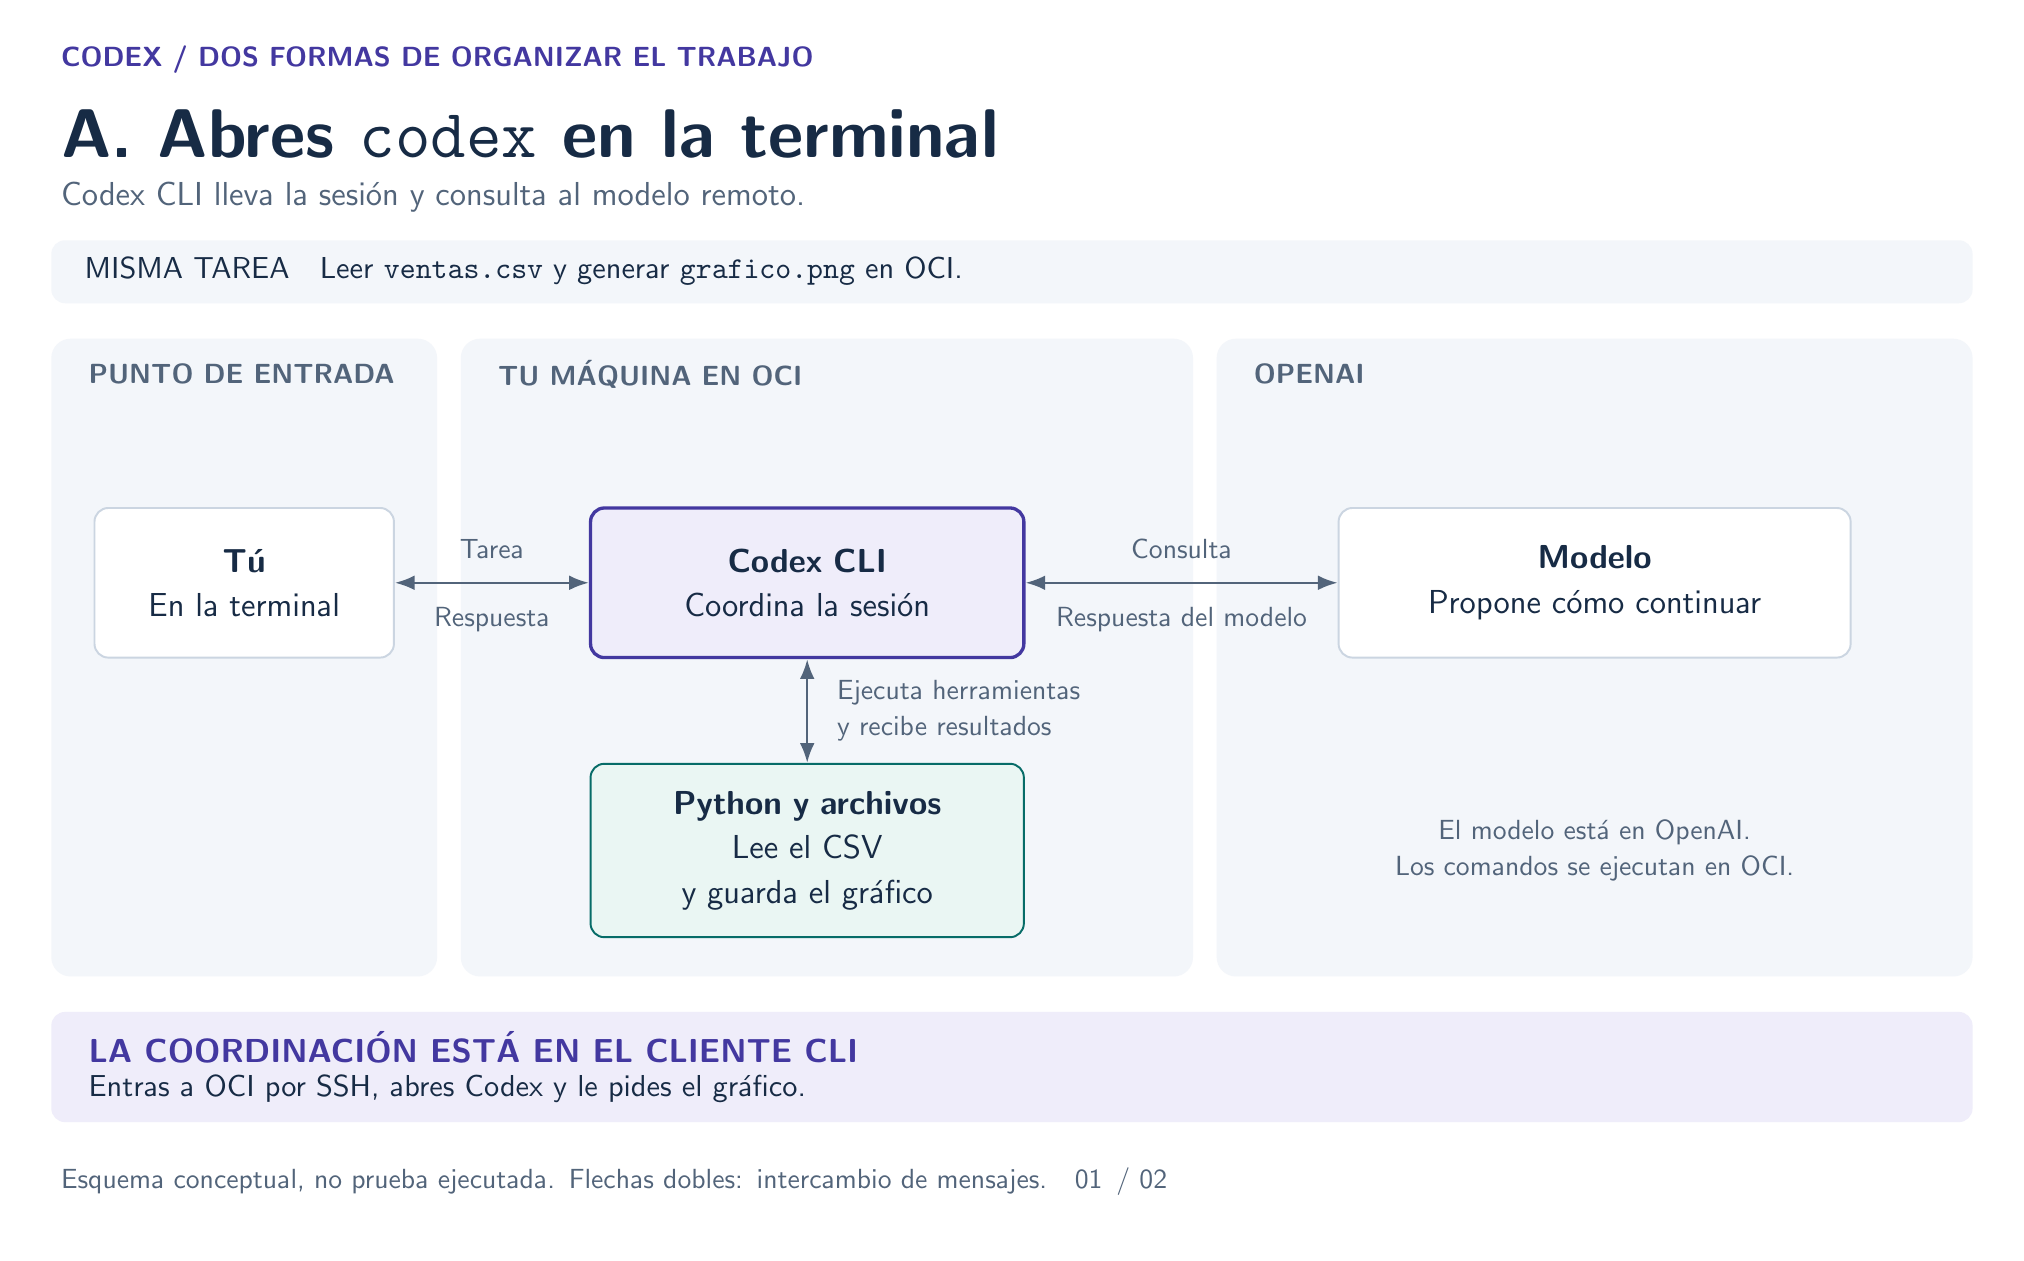
\begin{tikzpicture}
  \framebase{A. Abres \texttt{codex} en la terminal}{Codex CLI lleva la sesión y consulta al modelo remoto.}{01}
  \node[box,text width=3.1cm] (person) at (2.75,8.25)
    {\textbf{Tú}\\En la terminal};
  \node[coordinator] (cli) at (9.9,8.25)
    {\textbf{Codex CLI}\\Coordina la sesión};
  \node[box,text width=5.8cm] (model) at (19.9,8.25)
    {\textbf{Modelo}\\Propone cómo continuar};
  \node[tool] (tools) at (9.9,4.85)
    {\textbf{Python y archivos}\\Lee el CSV\\y guarda el gráfico};
  \draw[link] (person.east) -- (cli.west)
    node[midway,above=5pt,label] {Tarea}
    node[midway,below=5pt,label] {Respuesta};
  \draw[link] (cli.east) -- (model.west)
    node[midway,above=5pt,label] {Consulta}
    node[midway,below=5pt,label] {Respuesta del modelo};
  \draw[link] (cli.south) -- (tools.north)
    node[midway,right=7pt,label,align=left] {Ejecuta herramientas\\y recibe resultados};
  \node[label,text width=6.8cm] at (19.9,4.85)
    {El modelo está en OpenAI.\\Los comandos se ejecutan en OCI.};
  \takeaway{LA COORDINACIÓN ESTÁ EN EL CLIENTE CLI}{Entras a OCI por SSH, abres Codex y le pides el gráfico.}
\end{tikzpicture}
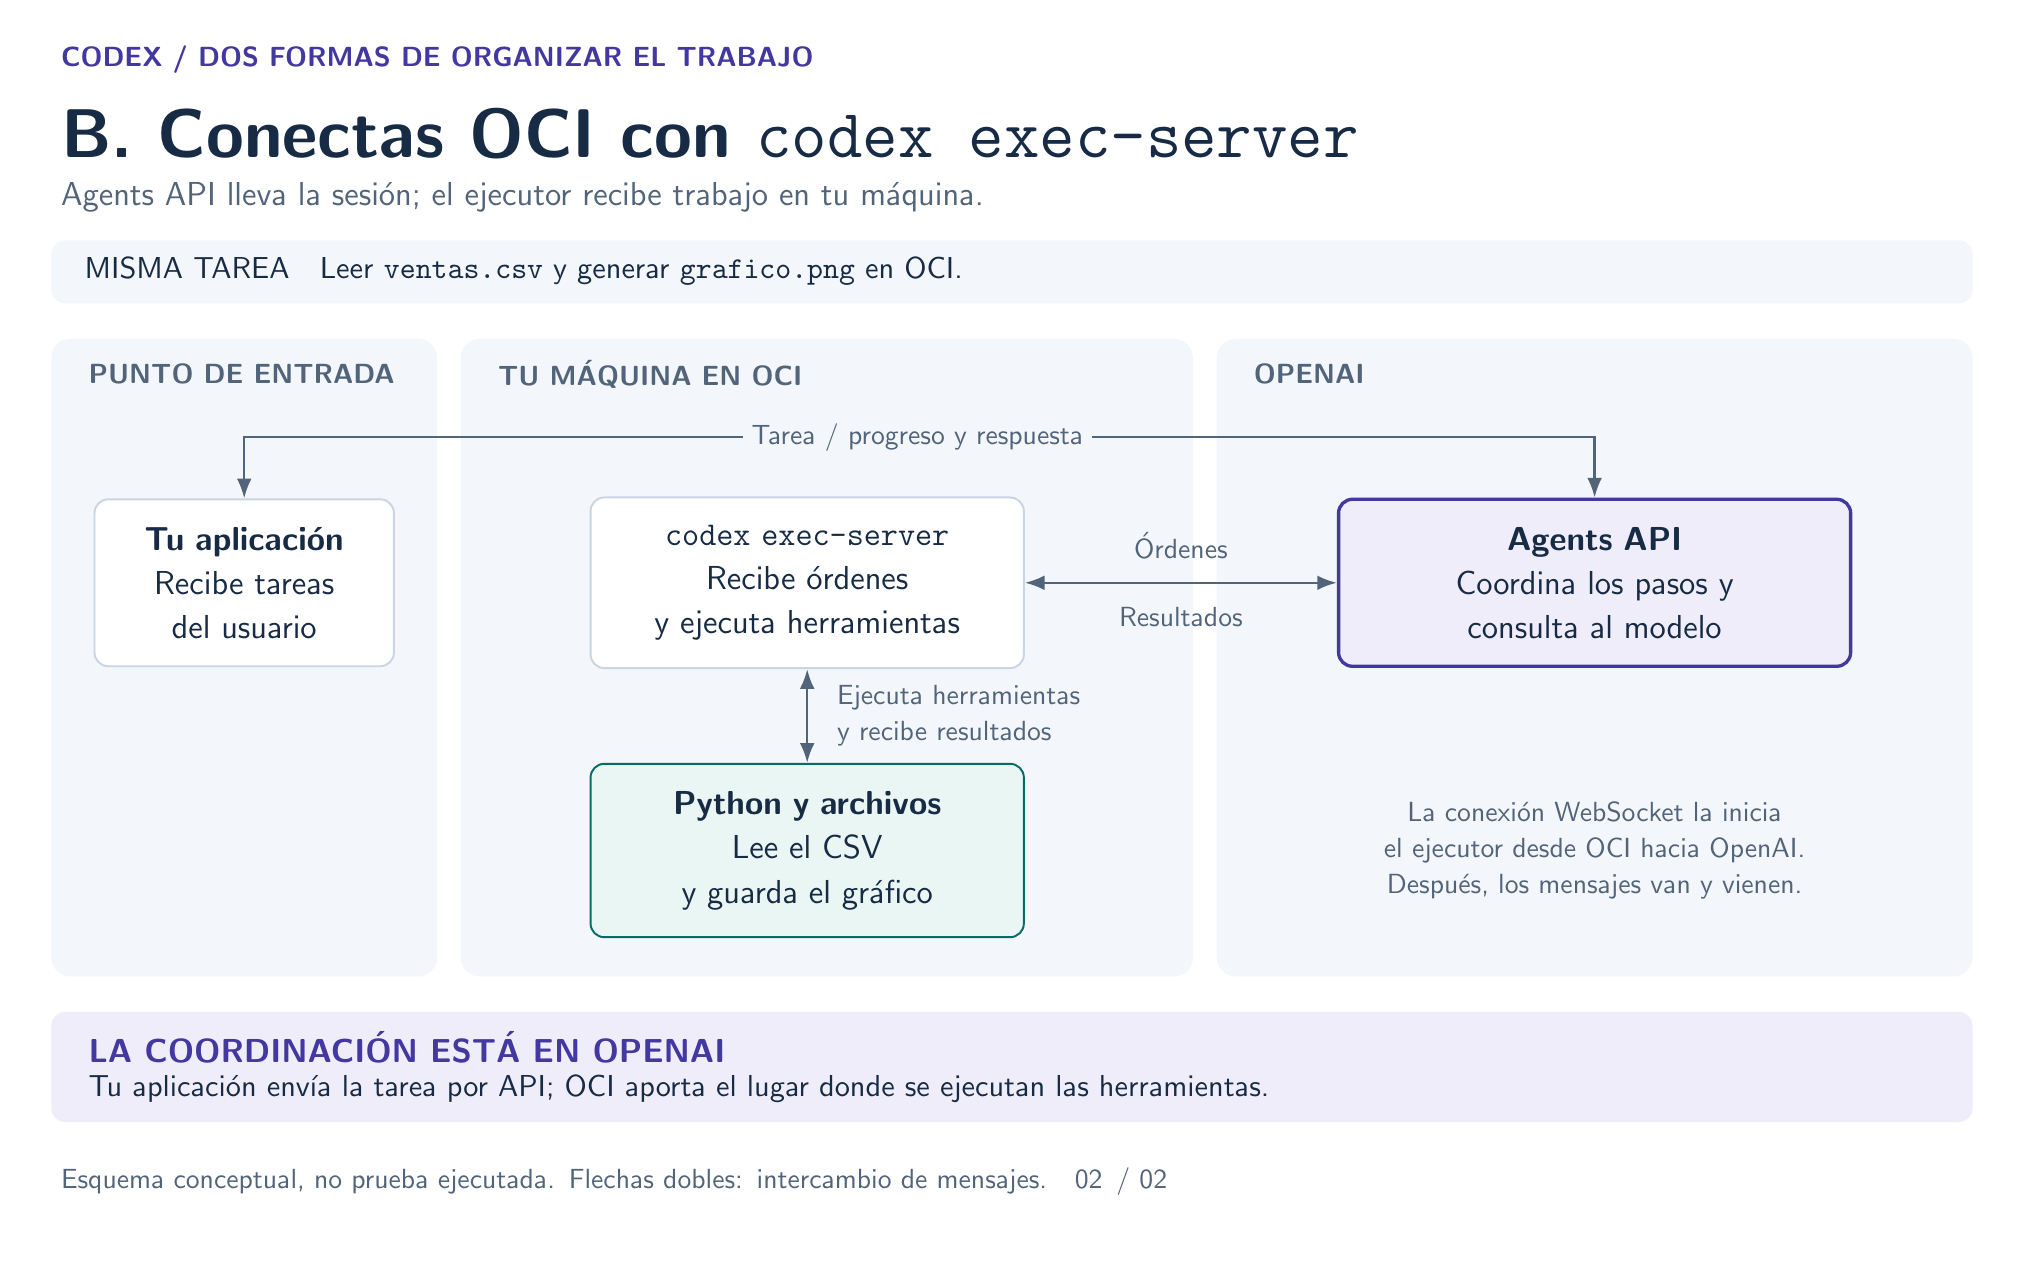
\begin{tikzpicture}
  \framebase{B. Conectas OCI con \texttt{codex exec-server}}{Agents API lleva la sesión; el ejecutor recibe trabajo en tu máquina.}{02}
  \node[box,text width=3.1cm] (app) at (2.75,8.25)
    {\textbf{Tu aplicación}\\Recibe tareas\\del usuario};
  \node[box] (executor) at (9.9,8.25)
    {\textbf{\texttt{codex exec-server}}\\Recibe órdenes\\y ejecuta herramientas};
  \node[coordinator,text width=5.8cm] (api) at (19.9,8.25)
    {\textbf{Agents API}\\Coordina los pasos y consulta al modelo};
  \node[tool] (tools) at (9.9,4.85)
    {\textbf{Python y archivos}\\Lee el CSV\\y guarda el gráfico};
  \draw[link] (app.north) -- (2.75,10.1) -- (19.9,10.1) -- (api.north);
  \node[label,fill=paper,inner sep=3pt] at (11.3,10.1) {Tarea / progreso y respuesta};
  \draw[link] (executor.east) -- (api.west)
    node[midway,above=5pt,label] {Órdenes}
    node[midway,below=5pt,label] {Resultados};
  \draw[link] (executor.south) -- (tools.north)
    node[midway,right=7pt,label,align=left] {Ejecuta herramientas\\y recibe resultados};
  \node[label,text width=7.7cm] at (19.9,4.85)
    {La conexión WebSocket la inicia\\el ejecutor desde OCI hacia OpenAI.\\Después, los mensajes van y vienen.};
  \takeaway{LA COORDINACIÓN ESTÁ EN OPENAI}{Tu aplicación envía la tarea por API; OCI aporta el lugar donde se ejecutan las herramientas.}
\end{tikzpicture}
\end{document}
